%
% Sección de composición del número de una tarjeta, capítulo de antecedentes.
% Proyecto Lovelace.
%

\section{Composición del número de una tarjeta}
\label{sec:composicion_tarjeta}

La información presentada a continuación puede consultarse con más detalle en
los siguientes documentos~\cite{iso_7812, iso_9362, pci_definitive_guide}.

Como se puede observar en la figura~\ref{figura:pan}, un número de tarjeta
\gls{gl:pan}, se compone por tres partes: el número identificador del emisor
(\gls{gl:iin}), el número de cuenta y un dígito verificador; la longitud del
\gls{gl:pan} puede variar e ir desde los 12 hasta los 19 dígitos. A
continuación se explica con más detalle cada uno de sus componentes

\subsection{Identificador del emisor}
El \gls{gl:iin} comprende los primeros 6 dígitos del número de
tarjeta. El primer dígito es conocido como \gls{gl:mii} y se encarga de
identificar la industria a la que pertenece el emisor; en la
tabla~\ref{tabla:mii}, se puede observar la relación entre el dígito y el giro.
El identificador del emisor provee, entre otros, los siguientes datos:

\begin{enumerate}
    \item Emisor de la tarjeta
    \item Tipo de la tarjeta (ej. crédito o débito)
    \item Nivel de la tarjeta (ej. clásica, Gold, Black)
\end{enumerate}

\begin{figure}
  \begin{center}
    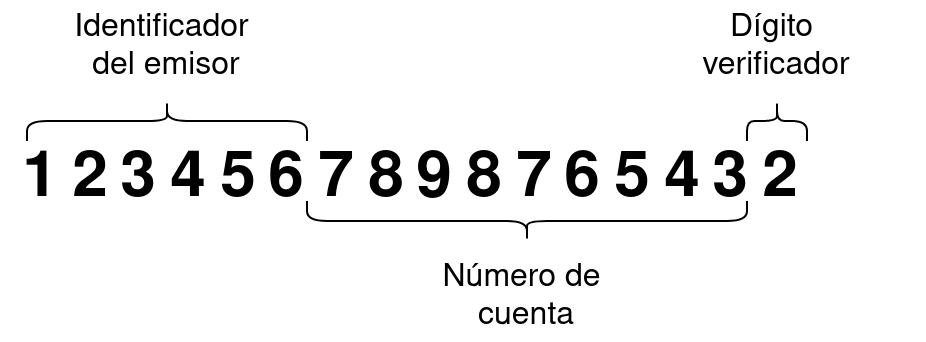
\includegraphics[width=0.6\linewidth]{diagramas/tarjeta}
    \caption{Componentes de un número de tarjeta.}\label{figura:pan}
   \end{center}
\end{figure}

\begin{table}
  \centering
  \begin{tabular}{ c|l }
    Dígito & Industria \\ \hline
    1, 2 & Aerolíneas \\
    3 & Viajes y entretenimiento (ej. American Express) \\
    4, 5 &  Bancos e industria financiera (ej. Visa, Mastercard)\\
    6 & Comercio (ej. Discover) \\
    7 &  Industria petrolera \\
    8 &  Telecomunicaciones \\
    9 &  Asignación nacional \\
    \end{tabular}
    \caption{Identificador de industria (\gls{gl:mii}).}\label{tabla:mii}
\end{table}

\subsection{Número de cuenta}
Todos los dígitos posteriores al \gls{gl:iin} y anteriores al último dígito,
comprenden el número de cuenta. La longitud de este puede variar, pero, máximo
comprende 12 dígitos, por lo que cada emisor tiene $10^{12}$ posibles números
de cuenta.

\subsection{Dígito verificador}
\label{sec:algoritmo_luhn}

Finalmente, se tiene el dígito verificador; este toma en cuenta todos los
dígitos anteriores y se calcula mediante el algoritmo de Luhn, que se describe
en~\ref{luhn:1}.

\begin{pseudocodigo}[%
    caption={Algoritmo de Luhn.},
    label={luhn:1}%
  ]
    entrada: número de tarjeta, compuesto desde 12 hasta 19 dígitos:
             $\{x_{n} x_{n-1} x_{n-2} \dots x_3 x_2 x_1\}$
    salida:  dígito verificador $x_1$.
    inicio
      Sean los conjuntos $x_{par}$ y $x_{impar}$:
          si $n$ es par:
              $x_{par} = \{x_2, x_4, x_6, \dots, x_n\}$
              $x_{impar} = \{x_3, x_5, x_7, \dots, x_{n-1}\}$.
          si_no:
              $x_{par} = \{x_2, x_4, x_6, \dots, x_{n-1}\}$
              $x_{impar} = \{x_3, x_5, x_7, \dots, x_n\}$.
      Obtener el doble de cada uno de los elementos del conjunto $x_{par}$:
        $x_{par doble} = \{2 \times x_2, 2 \times x_4, 2 \times x_6, \dots \}$.
      $\forall x_i \in x_{par doble} > 9$:
          $x_i = (x_i \mod 10) + 1 $
      Sumar los elementos de los conjuntos $x_{par doble}$ y $x_{impar}$.
      $x_1 = (S \times 9) \mod 10$
      Regresar $x_1$
    fin
\end{pseudocodigo}
